\documentclass[numsec,webpdf,modern,large,namedate]{oup-authoring-template}
\onecolumn
\usepackage{verbatim}
\usepackage{array}
\usepackage{booktabs}
\usepackage{fontspec}
\setmainfont{Libertinus Serif}
\begin{document}
\journaltitle{Journal of Language Evolution}
\copyrightyear{2026}
\pubyear{2026}
\appnotes{Paper}
\firstpage{1}
\title{Phylogenetic inference from cognate word forms}
\author[1,$\ast$]{David M. Goldstein}
\author[2]{Shawn H. McCreight}
\author[3]{\'{E}va Buchi}
\author[4]{John P. Huelsenbeck}

\address[1]{\orgdiv{Department of Linguistics}, \orgname{University of California, Los Angeles}\orgaddress{\street{UCLA}, \postcode{90095-1543}, \state{California}}}
\address[2]{\orgdiv{Nytril LLC}, \orgaddress{\street{2904 Horsehead Bay Dr. NW}, \postcode{98335}, \state{Washington}}}
\address[3]{\orgdiv{Centre national de la recherche scientifique}, }
\address[4]{\orgdiv{Department of Integrative Biology}, \orgname{University of California, Berkeley}\orgaddress{\street{UC Berkeley}, \postcode{94720}, \state{California}}}


\corresp[$\ast$]{David M. Goldstein \href{email:dgoldstein@humnet.ucla.edu}{dgoldstein@humnet.ucla.edu}}

\abstract{Linguistic phylogenies are commonly inferred from abstract cognate classifications that encode relationships among lexemes. Although widespread, this practice has well-recognized limitations: it discards the phylogenetic signal contained in segmental word forms; restricts the range of evolutionary questions that can be addressed; and treats cognacy judgments, which are hypotheses, as observed data. We introduce a comparative framework that addresses these limitations by modeling the evolution of aligned cognate word forms directly. Our approach adapts the TKF91 model of molecular evolution, originally developed to account for insertion and deletion events in DNA sequences, to the domain of linguistic data. By operating on segmental strings rather than abstract character codings, the framework enables phylogenetic inference from observable word forms and supports quantitative investigation of sound change. We demonstrate its utility through analyses that illuminate patterns of segmental stability and the evolution of phonological inventories.}

\keywords{Bayesian inference, Historical linguistics, Historical phonology, Phylogenetics, Romance}

\maketitle
\section{Introduction}
\label{PaperSections_Introduction}
Natural languages exhibit the property of descent with modification, which allows their histories to be represented as phylogenetic trees and inferred using methods originally developed in evolutionary biology \citep{Atkinson2005,Croft2008,Pagel2009,Borchesius2017,Bromham2017,Pagel2017}. Over the past two decades, such methods have become central to historical and evolutionary linguistics. Bayesian phylogenetic methods in particular are increasingly used to infer tree topologies, ancestral states, and divergence times \citep{Bouckaert2012,Bowern2012,Chang2015,Dunn2017,Sagart2019,Carling2021,Auderset2023,Heggarty2023}. Despite the undeniable advances of these methods, a foundational issue remains unresolved: the nature of the observations. We argue that modeling linguistic evolution as a sequence of explicit segmental events yields richer and more coherent inferences than current trait-based approaches. 

\subsection{Root-meaning traits}
\label{PaperSections_RootMeaningTraits}
Most linguistic phylogenies are inferred from abstract cognate relationships \citep{Gray2000,Holden2002,Ringe2002,Gray2003,Bouckaert2012,Bowern2012,Chang2015}. Cognates are linguistic units at different levels (e.g., segments, morphemes, words) that share a common ancestor. An example from the lexical domain is Spanish \textit{mano} ‘hand,’ French \textit{main}, and Italian \textit{mano}, which all descend from Proto-Romance */manu/. Four types of lexical cognacy have been identified in the literature \citep{Chang2015}, but phylogenetic studies rely overwhelmingly on one: root-meaning traits.

\begin{table}[t]
\centering
\caption{A root-meaning trait for the concept ‘hand.’ }
\setlength{\tabcolsep}{0pt}
\begin{tabular}{b{57.811pt} b{129.991pt} b{74.083pt} }
\specialrule{2pt}{0pt}{1.5pt}
Language & Phonemic Representation & Cognate Class\\
\specialrule{1pt}{0pt}{0pt}
English & /hænd/ & 0\\
German & /hant/ & 0\\
Dutch & /ɦɑnd/ & 0\\
French & /m\~{ɛ}/ & 1\\
Spanish & /mano/ & 1\\
Italian & /mano/ & 1\\
Russian & /ruka/ & 2\\
Polish & /rɛŋka/ & 2\\
Lithuanian & /ranka/ & 2\\
\specialrule{2pt}{1.5pt}{0pt}
\end{tabular}

\label{CognateCoding}
\end{table}

Root-meaning traits encode the ancestral relationships of the root of the most semantically general and stylistically neutral word associated with a given concept, such as ‘hand’ \citep{Heggarty2023}. The concepts are drawn from a restricted subset of the lexicon commonly referred to as the “basic vocabulary,” which includes terms for body parts, basic actions, natural phenomena, and other central domains of daily life that are assumed to be comparatively resistant to borrowing and replacement. These basic vocabulary items are typically organized into Swadesh lists, which now exist in several versions \citep{Tadmor2010}. 

Table$~$\ref{CognateCoding} presents a root-meaning trait for the concept ‘hand’ in a sample of Indo-European languages. Lexical items that descend from a common ancestor are grouped into the same cognate class, with class membership determined on the basis of regular sound correspondences. The resulting multistate cognate classifications are typically recoded as a set of binary characters, where 0 and 1 indicate the absence or presence, respectively, of a lexeme belonging to a given cognate class. These binary values constitute the observed data used for subsequent phylogenetic inference. 

Despite their widespread use, root-meaning traits exhibit several well-known limitations. The most serious is that the reduction of word forms to abstract cognate classes results in substantial information loss. For example, the lexemes for ‘hand’ in Spanish, French, and Italian are assigned the same state in Table$~$\ref{CognateCoding}. Since this representation exhibits no variation across these languages, no inferences can be drawn about their historical relationships. The segmental forms themselves, however, preserve phylogenetic signal: French /m\~{ɛ}/, Spanish /mano/, and Italian /mano/ each represent distinct reflexes of Latin /manum/. Standard trait-based methods in linguistic phylogenetics are not designed to incorporate such fine-grained segmental divergence into the inference process. 

Second, since root-meaning traits are analyzed analogously to morphological characters in biology \citep{Lewis2001}, they inherit the same methodological constraints. (i) The state labels, whether binary or multistate, are arbitrary and carry no intrinsic interpretation beyond distinguishing cognate classes. Consequently, linguistic phylogenetic analyses are effectively limited to models with symmetric transition rates, so that the likelihood is invariant to permutations of the state labels. That is, the probability of the data must remain unchanged if 0s and 1s are interchanged. (ii) Moreover, state labels are not comparable across lexical items. State 0 for one concept does not correspond to state 0 for another, which precludes pooling information across characters to estimate shared evolutionary dynamics. (iii) Invariant root-meaning traits (those exhibiting a single state across all languages) are relatively rare. Likelihood calculations must therefore condition on the exclusion of constant patterns from the data matrix. As a result, phylogenetic analyses based on such traits are largely confined to estimating tree topology and divergence times, while providing limited access to the dynamics of segmental change. 

Third, recoding multistate cognate relationships as binary characters induces statistical dependencies among the resulting variables. For any given concept, the presence of one cognate class in a language entails the absence of the others, except in cases of polymorphism. However, the continuous-time Markov models typically employed assume that characters evolve independently and identically distributed (i.i.d.). Binary characters derived from multistate cognate data violate this independence assumption. 

Finally, cognate-class assignments such as those in Table$~$\ref{CognateCoding} are treated as observed data, even though they are inferred. Cognacy judgments are hypotheses about ancestral relationships among lexical items and cannot be observed any more than a phylogenetic tree can. This practice sits uneasily with the principles of Bayesian inference, under which posterior distributions are conditioned on observable data. Our approach mitigates this tension by conditioning inference on attested word forms rather than abstract cognate classes. The selection of word forms, however, remains guided by prior assumptions of cognacy. 

\subsection{The TKF91 approach}
\label{PaperSections_TKF91Approach}
\begin{figure*}[b]
\centering
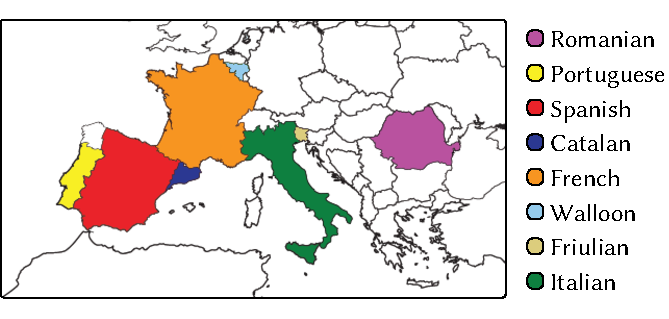
\includegraphics[width=304.95pt]{Figures/LanguageDistribution.pdf}
\caption{Approximate geographic distribution of the Romance languages in the study group.}
\label{LanguageDistribution}
\end{figure*}

We introduce an approach to linguistic phylogenetics in which the observations are aligned cognate word forms \citep{BouchardCote2013,Abner2024}. The segmental evolution of these forms is modeled as a continuous-time Markov process that permits three types of instantaneous events: (i) substitution of one segment by another; (ii) insertion of a segment; and (iii) deletion of a segment. This framework enables analysis in a manner directly analogous to molecular phylogenetic inference. The model, first introduced by \citet{Thorne1991}, is known in the molecular evolution literature as TKF91. Just as nucleotides are treated as equivalent states irrespective of genomic position, our method treats segments as equivalent states across words. This permits estimation of event rates by pooling information across lexical items and segmental positions. By operating directly on segmental strings, the approach overcomes the principal limitations of trait-based coding. It preserves segmental structure, avoids arbitrary state labels, accommodates invariant data, and conditions inference on observable word forms. 

Although the TKF91 model can be used for tree estimation, we focus on its capacity to estimate rates of change among segments, a central question in both linguistic theory and phonological typology. Several quantitative measures of diachronic segment stability have been proposed \citep{Wichmann2009,Moran2018,Moran2021}, but these approaches are not embedded within an explicit phylogenetic framework and do not model segment-to-segment transitions. A key advantage of our method is that it accommodates a broad class of transition models unconstrained by arbitrary state codings. We demonstrate the power of the TKF91 model with a sample of eight Romance languages together with Latin. The analysis yields three principal findings concerning sound change from Latin to Romance. First, vowels exhibit greater diachronic volatility than consonants. Second, models that parameterize transition rates over phonological natural classes provide a substantially better fit than simpler alternatives. Third, the inferred equilibrium frequencies indicate a disproportionate representation of stops and short vowels in Romance lexical forms relative to other segment classes. 

The remainder of this paper is structured as follows. Sections \ref{PaperSections_Data} and \ref{PaperSections_MethodsSection} describe the data and methodological framework. Section$~$\ref{PaperSections_Results} presents the empirical results. Section$~$\ref{PaperSections_DiscussionSection} situates these results within historical phonology and phonological typology and compares our approach to the other views of sound change. Section$~$\ref{PaperSections_Conclusion} concludes with a summary of the principal contributions and outlines directions for further development of the TKF91 approach. 

\section{Data}
\label{PaperSections_Data}
The dataset consists of cognate word forms drawn from a sample of eight Romance languages and Latin, whose geographic distribution is presented in Figure$~$\ref{LanguageDistribution}. The word forms are cognate in the traditional sense: they descend from a common ancestor \citep[p. 201]{Chang2015}. In contrast to root-meaning traits (such as the one illustrated in Table$~$\ref{CognateCoding}), cognacy does not depend on semantic equivalence. For instance, the Latin adjective \textit{gravis} means ‘heavy,’ but French \textit{grave} means ‘serious.’ Despite this semantic divergence, they are assigned to the same cognate set because they are segmentally homologous. 

\begin{table}[tb]
\centering
\caption{Manual alignment of the words for the concept ‘what.’ }
\setlength{\tabcolsep}{0pt}
\begin{tabular}{b{49.066pt} b{106.543pt} b{46.997pt} }
\specialrule{2pt}{0pt}{1.5pt}
Language & Phonemic Representation & Alignment\\
\specialrule{1pt}{0pt}{0pt}
Latin & /kʷid/ & kʷ-id\\
Romanian & /ʧe/ & ʧ-e-\\
Portuguese & /kɨ/ & k-ɨ-\\
Spanish & /ke/ & k-e-\\
Catalan & /kɛ/ & k-ɛ-\\
French & /kwa/ & kwa-\\
Walloon & /kwɛ/ & kwɛ-\\
Friulian & /ʧe/ & ʧ-e-\\
Italian & /ke/ & k-e-\\
\specialrule{2pt}{1.5pt}{0pt}
\end{tabular}

\label{ManualAlignment}
\end{table}

Cognate sets were assembled as follows. We began by identifying basic-vocabulary items in Latin using the Swadesh 207-item list. Although cognates of any semantic domain could in principle have been selected, the Swadesh list was employed solely to minimize the likelihood of borrowing. For each Latin lexeme, corresponding cognates in the eight Romance languages were collected from etymological dictionaries. Forms identified as borrowings, whether from Latin or among Romance varieties, were excluded. The decision to anchor the dataset in Latin was motivated by practical considerations. Since we only used complete cognate sets, beginning with Latin maximized the chances of having cognates in all of the Romance languages in our sample. (In principle, incomplete cognate sets, i.e., those lacking a reflex in one or more languages, could be incorporated. However, restricting the dataset to complete sets simplifies parameter estimation and was therefore adopted for this initial investigation.)

The dataset comprises 102 cognate sets, totaling 918 word forms and 79 distinct segments distributed across 98 concepts. Word forms may be represented either phonetically or phonemically; in this study, we adopt phonemic representations for two reasons. First, detailed phonetic transcriptions are not consistently available, particularly for a corpus language such as Latin. Second, the current implementation of the model does not accommodate within-language phonetic variation. Accordingly, reliance on phonetic data would have necessitated selecting a single, potentially arbitrary, surface realization for each form. All representations are strictly segmental. Suprasegmental properties, including stress and syllable structure, are not encoded. Segments are transcribed using standard Unicode IPA conventions \citep{IPA1999}. 

Within each cognate set, word forms were manually aligned. An illustrative example is provided in Table$~$\ref{ManualAlignment} for the concept ‘what.’ Dashes (‘-’) indicate the absence of a segment homologous to one present in other forms. For example, the /i/ of Latin /kʷ-id/ corresponds to /wa/ in French and Walloon. To represent the emergence of /w/, an empty segmental position is introduced before the vowel in the remaining languages. As discussed in Section$~$\ref{PaperSections_MethodsSection}, however, these manual alignments serve only as initial configurations for the Markov chain Monte Carlo procedure. Inference does not condition on any fixed alignment and the posterior distribution integrates over alternative homology assignments. Accordingly, explicit gap symbols are not required elements of the input. 

Latin is a highly synthetic language in which most lexical items exhibit multiple inflected forms. For purposes of analysis, each lexical item in the dataset is represented by a single form. Verbs are represented by the present active infinitive. Nouns, adjectives, and pronouns are represented by singular forms in either the accusative or, less frequently, the nominative case, as these are the case forms directly continued in the Romance languages. The selection of citation form is not methodologically neutral, as it can influence estimated transition rates. For example, most masculine singular nominative adjectives in Latin end in /-us/, whereas feminine singular nominative adjectives end in /-a/. Systematic inclusion of feminine forms would increase the number of transitions originating in this vowel. 

The lexical histories of the Romance languages are complex \citep{Stefenelli1992,Dworkin2016b}, as they reflect not only vertical inheritance but also substantial borrowing both from within Romance and from Latin itself. Given this non-tree-like component of their evolution, one might question the suitability of Romance data for phylogenetic modeling. In fact, Romance cognates are particularly well suited to our objectives for two reasons. First, the dataset is restricted to basic vocabulary, a domain in which borrowing is relatively infrequent \citep{Tadmor2010,Carling2019}. $Second, the phonological development of the Romance languages, which are attested in written sources from as early as the 9^{th}$$ and 10^{th}$ centuries, is sufficiently well understood that borrowings and Latinisms can often be identified. All forms for which evidence of borrowing was detected were excluded. Romance cognates are thus appropriate for our analysis for the same reason that the traditional comparative method has successfully reconstructed Proto-Romance forms. For example, the \textit{Dictionnaire \'{E}tymologique Roman} \citep{Derom} reconstructs portions of the Proto-Romance lexicon from a dataset comparable in scope and design to ours. 

\section{Methods}
\label{PaperSections_MethodsSection}
A comprehensive account of the model specification and computational implementation is provided in the Supplemental Material. The discussion here summarizes the essential components of the framework and the structure of the empirical analyses. 

\subsection{Model and Statistical Inference}
\label{PaperSections_ModelInference}
We assume that the languages in our sample are related by an unknown phylogenetic tree, $\Psi = (\tau , \nu )$, which encodes both their branching structure $(\tau )$ and the expected number of phonemic transition events $\nu $ along each branch. Evolution of word forms along the tree is modeled under TKF91 \citep{Thorne1991}, an event-based continuous-time process in which three instantaneous operations are permitted: segmental substitution, insertion, and deletion. Insertions and deletions occur at rates $\lambda $ and $\mu $, respectively, subject to the constraint $\lambda < \mu $. Segmental substitution is modeled as a continuous-time Markov process whose states correspond to phonemes (the inventory comprises 79 distinct segments). All pairwise substitution rates are specified by the rate matrix $\mathbf{Q}$, which is governed by parameters $\textit{$\theta$}$. 

\begin{table}[tb]
\centering
\caption{Model: “Natural Class”}
\setlength{\tabcolsep}{0pt}
\begin{tabular}{b{73.725pt} b{116.995pt} }
\specialrule{0.75pt}{0pt}{0pt}
Long Vowel & eː oː uː aː iː øː\\
Nasal Vowel & \~{ɐ}w \~{ɛ} ẽ \~{ɑ} \~{ɐ} \~{ɔ} \~{o} ĩ ũ \~{œ} \~{ɐ}j\\
Diphthong & o̯a ɨj ɨw ɔj au̯ ej ɛj e̯a aj oj ɐj\\
Short Vowel & o i a ə ɐ ɔ e u ɨ y ɛ œ ɑ ø\\
Nasal Consonant & m n ɲ ŋ\\
Liquid & l ʎ r ɾ ʁ ʀ\\
Approximant & j ɥ w\\
Affricate & ʧ ʦ ʤ\\
Fricative & ʃ x v f s h ʝ z ʒ $\theta$ ɣ\\
Stop & d k c p b t ɡ ɡʷ kʲ kʷ\\
\specialrule{0.75pt}{0pt}{0pt}
\end{tabular}

\label{PartitionAssignments}
\end{table}

Parameter estimation is conducted within a Bayesian framework, with inference based on the joint posterior distribution of all model parameters: 

\begin{align}
f(\Psi , \lambda , \mu , \textit{$\theta$}\vert \mathbf{S})= \frac{f(\mathbf{S}\vert \Psi , \lambda , \mu , \textit{$\theta$}) f(\Psi , \lambda , \mu , \textit{$\theta$})f(\mathbf{S})}{f(\mathbf{S})}
\end{align}

$\mathbf{S}$ denotes the observed segmental sequences of the cognate word forms. The likelihood function, $f(\mathbf{S}\vert \Psi , \lambda , \mu , \textit{$\theta$})$, is evaluated using the dynamic programming algorithm of \citet{Lunter2003}. Prior distributions for most parameters follow conventions standard in phylogenetic modeling. The insertion and deletion rate parameters, however, are assigned independent exponential priors subject to the constraint $\lambda < \mu $. An alignment of length $L$ is assigned a geometric prior with parameter $\lambda / \mu $. Under the TKF91 process, the equilibrium distribution of alignment lengths is geometric with parameter $\lambda / \mu $, which motivates this choice. A more principled alternative would specify a fully generative prior over alignments conditional on the insertion and deletion rates, derived directly from the TKF91 process. The development of such priors for segmental homology structures remains an important objective for future research. 

The posterior distribution is approximated numerically using Markov chain Monte Carlo, or MCMC \citep{Metropolis1953,Hastings1970}. We construct a Markov chain whose state space consists of the full set of model parameters and whose stationary distribution coincides with the posterior distribution of interest. After convergence, the samples drawn from this chain constitute dependent but valid draws from the posterior. In addition to phylogenetic parameters, the MCMC algorithm jointly samples segmental alignments \citep{Lunter2005a}. 

Segmental substitution is parameterized with reference to phonological natural classes, which are defined as sets of segments sharing phonetic features. The segment inventory is exhaustively partitioned into ten such classes, listed in Table$~$\ref{PartitionAssignments}. Under the Natural Class model, transition rates are allowed to vary across these ten classes. The model includes 79 parameters governing the equilibrium distribution and 80 parameters specifying exchange rates among natural classes. Equilibrium frequencies are treated as random variables with a flat Dirichlet prior. 

\subsection{Modeling linguistic history with cognate word-forms}
\label{PaperSections_CognateWordForms}
Working with cognate word forms presents specific methodological challenges, most notably the alignment of homologous segments across languages. In molecular phylogenetics, fine-grained homology among nucleotides is typically inferred using automated sequence-alignment algorithms. Even with long nucleotide sequences, however, alignment uncertainty can be substantial \citep{Wong2008}. This problem is amplified in lexical data, where word forms often contain only a small number of segments. To accommodate this uncertainty, we marginalize over possible segmental alignments rather than conditioning on a single fixed alignment. Concretely, all candidate alignments are integrated over, each weighted by its probability under the model. This integration is achieved within a Bayesian framework using MCMC, which jointly samples model parameters and segmental alignments in proportion to their posterior probabilities.

\subsection{Models of segmental change}
\label{PaperSections_SegmentModels}
\begin{figure}[tb]
\centering

\includegraphics[width=480.938pt]{Figures/ConceptEncoding.pdf}
\caption{The concept ‘mountain’ as coded in the data file.}
\label{ConceptEncoding}
\end{figure}

We evaluate three models of segmental change. $\textit{M}_1$ is isomorphic to the Jukes-Cantor model of DNA sequence evolution \citep{Jukes1969}, which specifies equal transition rates among all pairs of states, with substitutions occurring according to a Poisson process (hereafter the ‘Poisson’ model). $\textit{M}_2$, corresponds to the Felsenstein model \citep{Felsenstein1981}, in which the substitution rate from one segment to another is proportional to the equilibrium frequency of the destination segment. Finally, $\textit{M}_3$, the Natural Class model, partitions segments into articulatorily defined natural classes and permits distinct rates of change within and between these classes. Model complexity differs substantially across these specifications. $\textit{M}_1$ contains no free parameters. $\textit{M}_2$ includes 78 free parameters corresponding to the equilibrium frequencies (one fewer than the number of segments). The Natural Class model, $\textit{M}_3$, has 55 additional rate parameters governing transitions among natural classes, which yields a total of $78+ 55= 133$ free parameters.

\subsection{Data Curation and Analysis}
\label{PaperSections_DataCuration}
All analyses are orchestrated by a control program written in the Nytril programming language \citep{Nytrilprogram}. We developed an automated experimental pipeline comprising a reusable IPA library, curated word-form datasets, data-validation routines, typeset output generation, and input-file construction for the MCMC engine, which is implemented in C++. 

\begin{figure}[b]
\centering
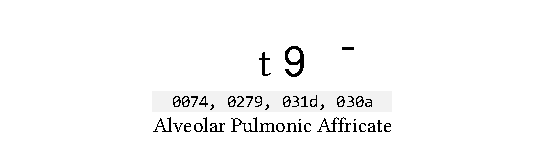
\includegraphics[width=249.375pt]{Figures/SegmentEncoding.pdf}
\caption{The IPA-Unicode encoding of a segment.}
\label{SegmentEncoding}
\end{figure}

Word forms from the nine languages are organized hierarchically by concept and cognate class. Figure$~$\ref{ConceptEncoding} illustrates the raw encoding for the concept ‘mountain.’ A central technical challenge arises from the fact that IPA transcriptions are encoded in Unicode (UCS), which cannot be represented in single-byte encodings such as ASCII. Accordingly, all data are stored in UTF-8, a cross-platform multibyte encoding of UCS. To ensure reliable string comparison, diacritic composition must be standardized; we adopt Unicode Normalization Form C, although consistency across files is the critical requirement. Moreover, a single IPA segment may consist of multiple UCS code points, so the correspondence between characters and phonological segments is not one-to-one. 

Figure$~$\ref{SegmentEncoding} provides an example of a complex encoding in which the grey numerals indicate hexadecimal UCS code points for base characters and diacritics. Since the analysis operates at the segmental level, a parser converts each word string into an array of segment objects. These objects are implemented in a reusable library that associates each segment with linguistic features. Subsequent processing steps operate on abstract properties such as ‘vowel’ and ‘nasal,’  rather than on raw character strings. 

Following parsing, the control program aggregates and partitions the data and generates the input required for Bayesian inference under the TKF91 model. The MCMC analysis runs for 5,000,000 cycles, with independent runs performed to assess convergence. Samples taken during the first 15,000 cycles of the chain are discarded as burn-in. Upon completion, posterior samples are imported back into the control program for post-processing. All tables, trees, and graphical outputs are generated automatically from the MCMC results and integrated with author-supplied narrative to produce the final manuscript and supplementary materials. 

\section{Results}
\label{PaperSections_Results}
\subsection{Phylogeny}
\label{PaperSections_PhylogenyResults}
\begin{figure}[tb]
\centering
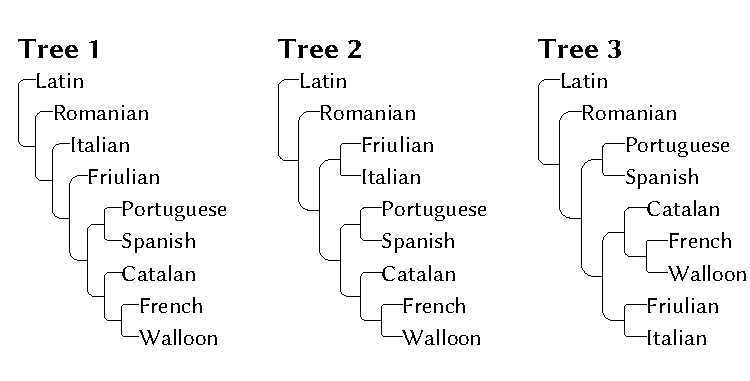
\includegraphics[width=242pt]{Figures/ModelTreesUsed.pdf}
\caption{Model trees used in all analyses}
\label{ModelTreesUsed}
\end{figure}

All model parameters are treated as random variables endowed with prior distributions. The tree topology describing the relationships of the languages is likewise modeled as a random variable under a uniform prior over all possible topologies. As outlined in Section$~$\ref{PaperSections_ModelInference}, the posterior probability distributions of the model parameters are numerically approximate with MCMC. Across runs, a small set of topologies consistently achieved the highest posterior support. However, the MCMC sampler exhibited limited mixing over tree space: once a high-probability topology was located, the chain tended to remain trapped in its vicinity. 

In our implementation, parameters are updated in blocks, with each MCMC step randomly selecting a single component and proposing a modification to it. Within a given cycle, either the tree topology or the segmental alignment is updated, but not both simultaneously. This update scheme induces dependence between topology and alignment. As improved topologies were accepted, the sampled alignments increasingly adapted to the current tree stored in memory. Once the alignment became well-tuned to a particular topology, proposals involving alternative trees were rarely accepted, even when they would have been plausible under a different alignment configuration. 

This difficulty does not appear to have arisen in earlier applications of TKF91 \citep{Lunter2005a}, which analyzed an alignment of amino acid sequences. Our analysis of cognate data yielded insertion and deletion rates that were large relative to substitution rates: $\lambda = 0.243$ (0.217, 0.273) and $\mu = 0.298$ (0.266, 0.335), respectively. (Each credible interval contains the true parameter value with probability 0.950.) In approximate terms, this implies one insertion or deletion event for every two substitution events. Like substitution events, insertion and deletion events contribute phylogenetic signal. In contrast to the earlier analysis of amino acid sequence data, the insertion and deletion events exerted substantial influence on tree support and their contribution varied with the sampled homology assignments. 

\begin{figure*}[b]
\centering
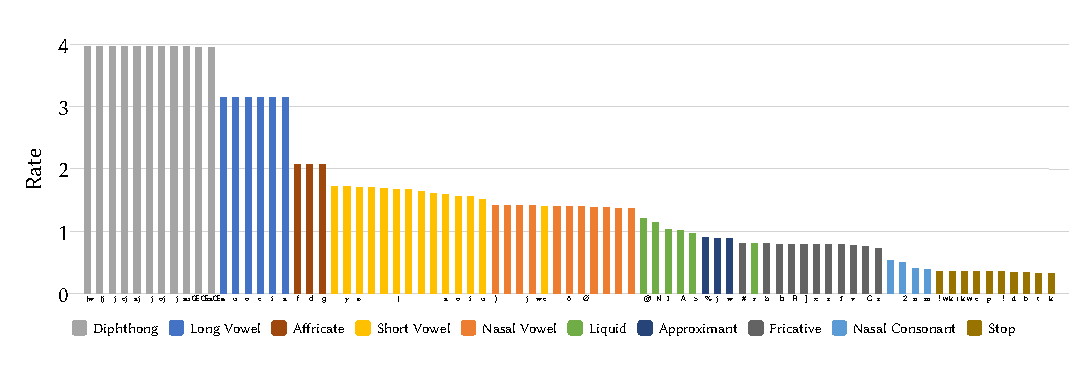
\includegraphics[width=495.9pt]{Figures/QRatesDiagonal.pdf}
\caption{The rate of change when in a particular segmental state (or $- q_{ii}$)}
\label{QRatesDiagonal}
\end{figure*}

Subsequent analyses therefore condition on the three fixed topologies in Figure$~$\ref{ModelTreesUsed}. Although the diversification of Romance remains debated, many recent accounts posit Sardinian as the earliest branching lineage, followed by Romanian \citep{Hall1950,Hall1976,Dardel1985,Swiggers2001,Vallejo2012,Buchi2015,Dworkin2016a}. Since Sardinian is not in our sample, Romanian occupies the earliest branching position in each topology in Figure$~$\ref{ModelTreesUsed}. The internal structure of the subtrees varies across the three configurations, but Spanish and Portuguese consistently form a clade, as do Catalan, French, and Walloon. 

The relationship between Classical Latin, Vulgar Latin, Proto-Romance, and the Romance languages remains the subject of ongoing debate \citep{Posner1996,Harris2003,Chang2015,Heggarty2023,Goldstein2024}. A central issue is whether Latin (Classical or Vulgar) is a sampled ancestor of the Romance languages or their sister lineage. For reasons of model tractability, we adopt the latter assumption and treat Latin as an outgroup. Tree models that incorporate sampled ancestors are considerably more complex than the framework employed here. This modeling choice does not exclude an ancestral interpretation, however: if the estimated branch length leading to Latin approaches zero, Latin is effectively positioned at the root of the Romance clade. 

\subsection{Model Comparison}
\label{PaperSections_ModelComparison}
\begin{align}
\textit{BF}= \frac{f(\mathbf{S}\vert \textit{M}_i)f(\mathbf{S}\vert \textit{M}_j)}{f(\mathbf{S}\vert \textit{M}_j)}
\end{align}

We assessed the relative fit of the three segmental-change models introduced in Section$~$\ref{PaperSections_MethodsSection} using Bayes factors. The Bayes factor is the ratio of the marginal likelihoods of the models: 

Ratios greater than one indicate evidence in favor of model $\textit{M}_i$. Since the candidate models are nested, we computed the Bayes factor via the Savage-Dickey density ratio \citep{Dickey1971}, which evaluates the ratio of posterior to prior densities at the parameter restriction that reduces the richer model to the simpler one. The Natural Class model explains the data substantially better than the two simpler alternatives. The log Bayes factors are $\ln \textit{BF}_{12}= -1074.2$ and $\ln \textit{BF}_{23}= -117.3$, comparing $\textit{M}_1$ to $\textit{M}_2$ and $\textit{M}_2$ to $\textit{M}_3$, respectively. This difference constitutes overwhelming support for the more parameter-rich Natural Class model \citep{Jeffreys1939}. 

\subsection{Segmental Change}
\label{PaperSections_WordTransformation}
Figure$~$\ref{QRatesDiagonal} presents the absolute values of the diagonal entries of the substitution rate matrix estimated under the Natural Class model. These diagonal elements provide a measure of segmental volatility, as each diagonal element equals the sum of transition rates from a given segment to all alternative segments. When the process is in segment $i$, the value $- q_{ii}$ represents the instantaneous rate at which it changes state. Higher values therefore correspond to shorter expected residence times and greater diachronic instability. Several segmental classes in Figure$~$\ref{QRatesDiagonal} appear to share identical rates (e.g., diphthongs, long vowels, affricates, and nasal vowels). This visual uniformity is an artifact of scale rather than exact equality. Although the rates in these classes are distinct, they are sufficiently small to be indistinguishable at the resolution of the plot. 

\begin{figure}[b]
\centering
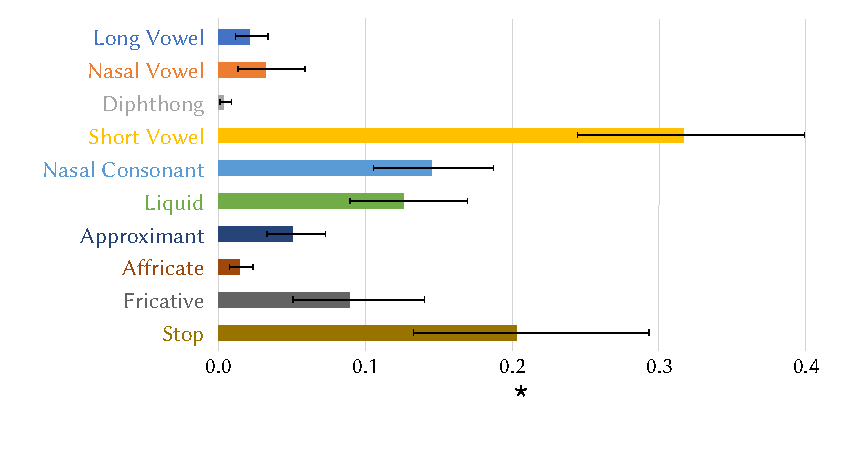
\includegraphics[width=300pt]{Figures/EquilibriumCharts.pdf}
\caption{The equilibrium frequencies $\pi $ of each natural class}
\label{EquilibriumCharts}
\end{figure}

The most salient pattern in Figure$~$\ref{QRatesDiagonal} is the clear separation between vowels and consonants. With the exception of affricates, vowels exhibit the highest volatility, and within the vocalic domain diphthongs and long vowels are particularly unstable. By contrast, the most stable segments are consonants, with stops displaying the lowest overall rates of change. Rates also cluster tightly within natural classes: long vowels, affricates, fricatives, short vowels, nasal vowels, nasal consonants, and stops each form coherent groups. Two segments depart from this pattern: the liquid /r/, which clusters with the fricatives, and the mid-front vowel /e/, which patterns with the nasal vowels. These patterns arise from the interaction between class-specific exchangeability parameters and the distribution of equilibrium frequencies. When equilibrium frequencies are relatively homogeneous within a class, the corresponding $- q_{ii}$ values tend to be similar. The clustering observed in Figure$~$\ref{QRatesDiagonal} thus reflects both the structural constraints of the model and regularities present in the empirical data. 

\begin{figure*}[b]
\centering
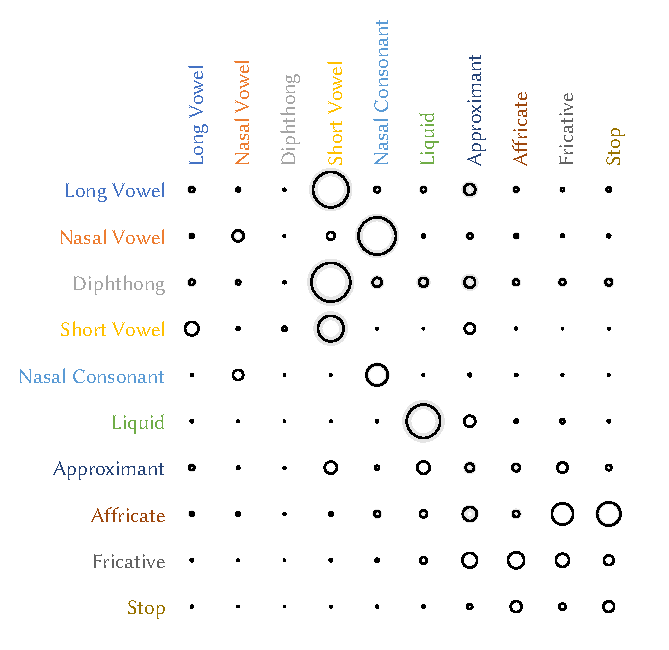
\includegraphics[width=304.95pt]{Figures/RateChart.pdf}
\caption{The average rates of change between and within the ten groups of the Natural Class model. Circle area is proportional to the rate of change between groups ($q_{ij}$). Shaded area represents the 95\% credible interval. }
\label{RateChart}
\end{figure*}

Figure$~$\ref{EquilibriumCharts} displays the estimated equilibrium frequencies under the Natural Class model $\textit{M}_3$. These frequencies enter the likelihood in two ways. First, they determine the prior distribution over segmental states at the root of the tree. Second, in models $\textit{M}_2$ and $\textit{M}_3$, they scale substitution rates so that transitions into a segment are proportional to its equilibrium frequency. Accordingly, transitions into liquids$~$(0.188), short vowels$~$(0.110), and nasal consonants$~$(0.0758) exhibit the highest estimated rates, which reflects their comparatively large equilibrium weights. More broadly, the inferred equilibrium distribution closely mirrors the empirical segment frequencies observed in the dataset. 

\begin{figure*}[b]
\centering
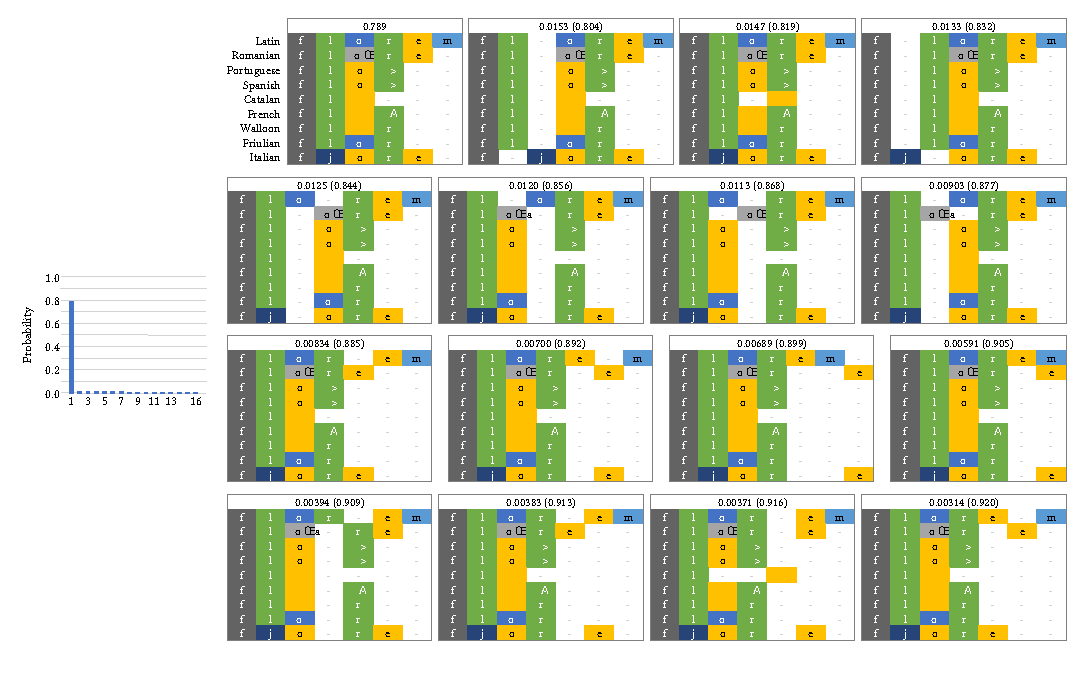
\includegraphics[width=495.9pt]{Figures/AlignmentExample1.pdf}
\caption{Segments are colored according to natural class. Dashes denote gaps where there is no homologous segment for the alignment position. The alignments are ordered from the highest posterior probability (top-left alignment) to the lowest posterior probability (bottom-right alignment) in row order. }
\label{AlignmentExample1}
\end{figure*}

Figure$~$\ref{RateChart} shows the estimated substitution rates among the 10 groups of the Natural Class model. Within-class exchange rates are elevated for short vowels, nasal consonants, and liquids. Relative to an equal-rates Poisson model, the within-class rates are 0.33, 1.63, 0.05, 8.59, 5.91, 14.70, 0.90, 0.52, 2.28, and 1.52 times larger for long vowels, nasal vowels, diphthongs, short vowels, nasal consonants, liquids, approximants, affricates, fricatives, and stops, respectively. Thus within-class exchange falls below the equal-rates expectation for long vowels, diphthongs, approximants, and affricates, while it exceeds expectation for nasal vowels, short vowels, nasal consonants, liquids, fricatives, and stops. Exchange rates between long vowels and short vowels, and between diphthongs and short vowels, exceed the corresponding within-class rates, a tendency discussed in section 5.2 below. Overall, 60.0\% (6 out of 10) of within-class transitions exceed the equal-rates expectation, compared to 23.3\% (21 out of 90) of transitions between distinct classes. This asymmetry indicates that, although not universal across classes, substitution rates are more frequently higher within natural classes than between them. This asymmetry reinforces the conclusion that segments are more likely to change within their own natural class than across class boundaries. 

\subsection{Segmental Alignments}
\label{PaperSections_WordSegmentRelationships}
\begin{figure}[b]
\centering
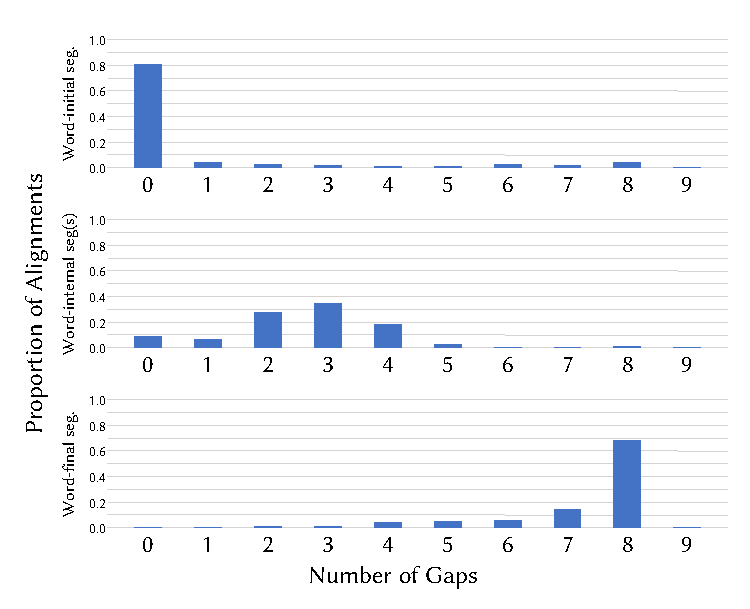
\includegraphics[width=300pt]{Figures/GappinessChart.pdf}
\caption{Distribution of alignment gaps across word positions for the 102 cognate sets analyzed in this study. The top panel shows the proportion of alignments with a given number of gaps at the word-initial segment, the middle panel at word-internal segments, and the bottom panel at the word-final segment. Since nine languages are analyzed, at most eight gaps can occur at a given position: a deletion event affecting all nine languages would not appear in the alignment and is explicitly conditioned on in the likelihood calculation \citep{Lunter2003}. Gaps increase systematically from initial to final position, with word-final segments exhibiting substantially higher deletion rates. A likelihood-ratio test rejects the null hypothesis that the gap distributions are identical across positions, ($\chi ^2= 425.62$, $d.f.= 16$, $p< 0.001$), which confirms a statistically significant positional asymmetry. }
\label{GappinessChart}
\end{figure}

In our framework, segmental homology across languages is treated as a latent random variable. Posterior uncertainty over alignments is summarized by constructing a credible set for each cognate word form. Alignments are ordered by posterior probability and the smallest set whose cumulative posterior mass reaches 0.95 is retained. Figure$~$\ref{AlignmentExample1} illustrates this procedure for the concept ‘flower’. Three general properties emerge. First, posterior mass is typically concentrated on a single dominant alignment. In the example shown, the highest-probability alignment alone accounts for 0.79 of the posterior. Second, insertion and deletion events occur disproportionately in word-final position, consistent with the distribution of gap frequencies shown in Figure$~$\ref{GappinessChart}. Third, segments from the same natural class tend to be assigned to the same column in the alignment. 

\begin{figure*}[b]
\centering
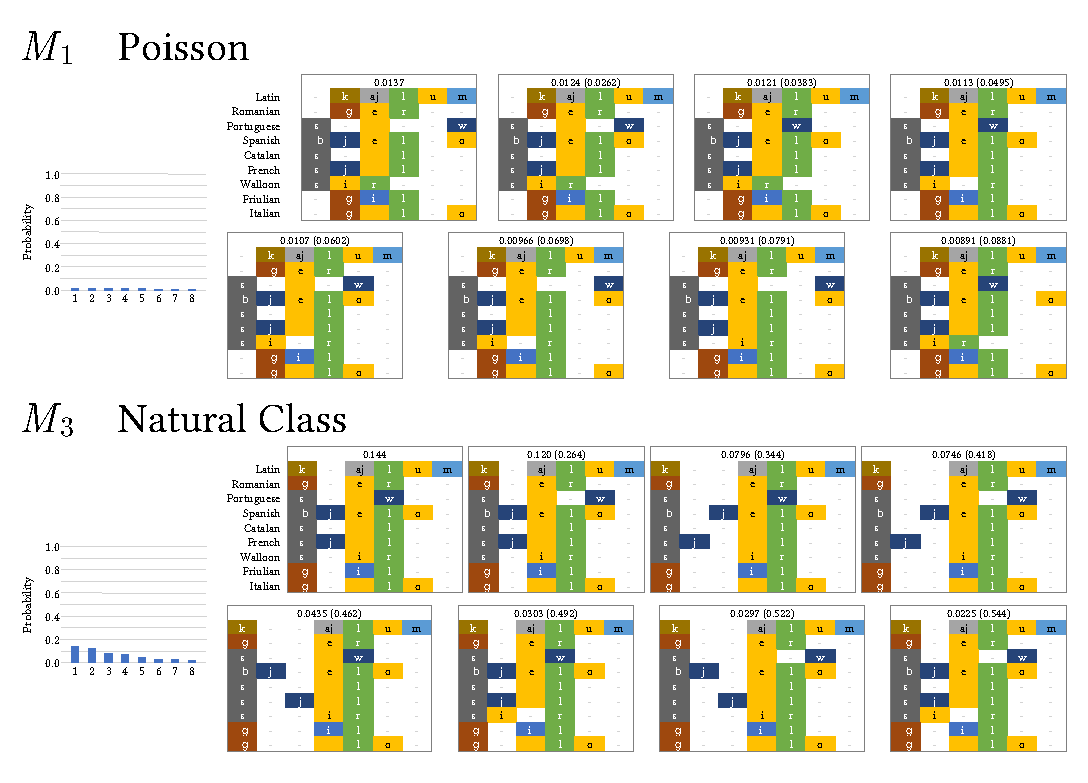
\includegraphics[width=495.9pt]{Figures/AlignmentExample2.pdf}
\caption{Alignments of highest posterior probability of the cognate for the concept ‘sky.’ The eight alignments under the $\textit{M}_1$ (Poisson model) account for 0.0881 posterior probability. The eight alignments under the $\textit{M}_3$ (Natural Class model) account for 0.544 posterior probability. }
\label{AlignmentExample2}
\end{figure*}

The posterior distribution over alignments is sensitive to the substitution model. Figure$~$\ref{AlignmentExample2} presents the 95\% credible set of alignments for the concept ‘sky’ under the Poisson and Natural Class models. Under the Poisson model, the credible set contains 1,363 alignments under the Poisson, whereas under the Natural Class model it contains only 226 alignments under the Natural Class. This reduction in alignment uncertainty accords with the substitution-rate structure estimated under the Natural Class model (Figure$~$\ref{RateChart}). For instance, transitions between /u/ and /o/ are assigned relatively high rates, whereas substitutions between consonants and /o/ are strongly disfavored. Consequently, the Poisson model frequently aligns consonants with /o/, while such configurations receive negligible posterior weight under the Natural Class model. 

\section{Discussion}
\label{PaperSections_DiscussionSection}
\subsection{Event-Based Modeling of Sound Change: The TKF91 Approach}
\label{PaperSections_OtherApproaches}
Theories of sound change exhibit substantial differences in their assumptions about units and mechanisms. One influential tradition treats phonemes as the primary units of change \citep{Bloomfield1933}. Under this view, sound change is abrupt and non-independent. For instance, a transition from /a/ to /o/ proceeds without intermediate stages and the shift is conceived as a single systemic event affecting all relevant lexical items simultaneously. Other approaches emphasize the role of phonetic factors, particularly acoustic and perceptual pressures, in driving change \citep{Ohala2003,Blevins2004a,Ohala2012}, while still others argue that sound change diffuses gradually through the lexicon in a process known as lexical diffusion \citep{Chen1975a,Phillips2015}. 

The TKF91 framework does not align fully with any single tradition, though it shares features with both phoneme-based accounts and lexical diffusion. Since the observations are phonemic strings, insertions, deletions, and substitutions operate over phonemes. Unlike classical historical models, however, changes are not treated as globally synchronized events. A shift from /a/ to /o/ is not modeled as a single transformation applied uniformly across the lexicon. Instead, a substitution rate is inferred from the observed homologies, which captures how frequently /a/ transitions to /o/ across cognate sets. In this respect, sound change is modeled as a stochastic process operating independently across lexical items. 

Our use of TKF91 parallels the approach of \citet{BouchardCote2013}, who likewise treat cognate word forms as the observed data. Their framework employs a string transducer model \citep{Holmes2001} to characterize segmental correspondences, which thereby accommodates context-dependent processes. By contrast, the current implementation of TKF91 does not incorporate contextual conditioning. Its advantage lies elsewhere: TKF91 is an explicitly historical, event-based model in which insertion, deletion, and substitution are well-defined stochastic events. The likelihood integrates over all possible sequences of such events that could have generated the observed forms in the nine languages. Since these events are parameterized by estimable rates, the model provides a direct quantitative account of segmental evolution. Even though it does not yet capture contextual phonological processes, its event-based structure offers a principled foundation for modeling sound change. 

A practical limitation of TKF91 is computational complexity. Likelihood evaluation scales exponentially with the number of taxa and word length, with complexity on the order of $O(2^{\textit{N}}L^{\textit{N}})$, where $\textit{N}$ denotes the number of tips and $L$ the geometric mean word length \citep{Lunter2003}. For linguistic datasets, this burden is mitigated by the brevity of word forms, typically $1\leq L\leq 10$. Nevertheless, alternative formulations can reduce computational cost. If insertion events are assumed to occur independently of word length, rather than at rate $\lambda (L+ 1)$ as in TKF91, the likelihood becomes linear in the number of taxa \citep{BouchardCote2013b}. This variant, known as the Poisson Indel Process (PIP), may be preferable for datasets comprising substantially larger language samples. Given that sampled alignments in our analyses exhibit comparable lengths, PIP constitutes a plausible direction for scaling the framework to broader comparative datasets. 

\subsection{Implications for Sound Change and Phonological Typology}
\label{PaperSections_InsightsSoundChange}
Traditional historical phonology is primarily concerned with identifying individual sound changes and establishing their relative chronology. By contrast, the TKF91 framework permits inference about broader systemic tendencies in the evolution of segmental inventories. We focus on three quantities that illuminate these tendencies: the diagonal elements of the substitution rate matrix, transition rates within and between natural classes, and the equilibrium distribution of segments. These quantities provide a quantitative characterization of sound change within an explicit phylogenetic model. 

As discussed in Section$~$\ref{PaperSections_MethodsSection}, the diagonal entries of the Q matrix measure the instantaneous rate at which a segment transitions to any other state, and thus provide an index of diachronic stability. The pronounced separation between vowels and consonants in Figure$~$\ref{QRatesDiagonal} aligns with established findings in Romance historical phonology. Among the major developments distinguishing Latin from the Romance languages is the loss of phonemic vowel length \citep{Janson1979,Loporcaro2015} and the early monophthongization of Classical Latin diphthongs \citep[p. 106]{Posner1996}. More broadly, our results accord with evidence that vowel inventories have evolved more rapidly than consonant inventories within Indo-European \citep[pp. 92--95]{Moran2021}. 

The present findings also intersect with work in phonological typology that seeks to identify core or stable segment inventories. The basic consonant inventory proposed by \citet{Nikolaev2020}, /p t k n l r/, is consistent with our results insofar as stops and nasals emerge as among the most stable classes. An even closer correspondence is found with the set of primal consonants identified by \citet{Bybee2022}, /p t k b d g m n ŋ s l/. Two distinctions, however, are crucial. First, primal consonants are defined in terms of their rarity as outputs of sound change, whereas the diagonal of the Q matrix measures the rate of transition away from a segment---that is, its stability as an input to change. Second, typological proposals aim to identify cross-linguistic universals, whereas our estimates characterize tendencies within Romance. The results therefore inform typological debates, but should not be interpreted as cross-linguistic universals. 

The average rates summarized in Figure$~$\ref{RateChart} provide a complementary perspective on segmental stability by comparing transitions within and between natural classes. Within-class rates exceed cross-class rates for short vowels, nasal consonants, and liquids. Liquids display the highest within-class rates, whereas diphthongs exhibit the lowest. A liquid is thus more likely to change into another liquid than into a segment of a different class, a pattern plausibly associated with processes such as liquid dissimilation, e.g., Latin \textit{arbor} > Spanish \textit{\'{a}rbol} \citep{Abrego2013,Mueller2013}. Transition rates between diphthongs and short vowels are the highest among all between-class rates, which is consistent with the reciprocal effects of vowel breaking and monophthongization in the history of Latin and Romance. More generally, the largest off-diagonal rates involve vowel classes, which reinforces the broader pattern of vocalic instability identified above. Elevated rates between nasal vowels and nasal consonants further reflects the development of nasalized vowels in French and Portuguese. 

The equilibrium frequencies in Figure$~$\ref{EquilibriumCharts} illuminate the distributional consequences of these historical processes. Short vowels and stops together account for more than half of all segments, which indicates a pronounced skew toward these classes. This distribution reflects the reduction of diphthongs and long vowels and the concomitant expansion of short vowels within Romance. 

Finally, model comparison provides quantitative support for the role of natural classes in sound change \citep[p. 201]{King1969}. Sound change frequently targets segments that share articulatory or acoustic properties, as exemplified by Grimm’s Law, which systematically affected theProto-Germanic reflexes of Proto-Indo-European stops. The superior fit of the natural-class model thus reinforces the long-standing view that phonetic grounding constrains the trajectory of phonological change. 

\subsection{Segmental Sampling}
\label{PaperSections_SegmentalSampling}
Under our framework, a new issue emerges: segmental sampling \citep{Dockum2019}. Specific sound changes can be pivotal for recovering tree topology, yet a dataset assembled on the basis of a Swadesh list does not ensure that such diagnostic patterns are adequately represented. For instance, Romanian merges Proto-Romance */ɔ/ and */o/ to /o/ and */ʊ/ and */u/ to /u/. By contrast, Italo-Western Proto-Romance (the common ancestor of the remaining languages in our sample) merges */ʊ/ and */o/ to /o/. Consequently, Latin \textit{buccam} ‘mouth’ and Romanian \textit{bucă} preserve /u/ against the /o/ reflex found, for instance, in Italian \textit{bocca}. This change constitutes key evidence for the placement of Romanian within the Romance tree \citep{Janson1979,Herman2000}. If such correspondences are underrepresented in the sample, the topology may be estimated incorrectly. A related issue concerns the representativeness of the segment-frequency distributions in Figure$~$\ref{SegmentOccuranceRates}. These distributions are derived from word forms sampled under specific selection criteria and may not faithfully approximate the segment frequencies of each language. Systematic discrepancies of this kind can bias estimates of substitution rates and, in turn, influence inferences about sound-change dynamics and phylogenetic structure. 

\subsection{Limitations of the Model}
\label{PaperSections_Limitations}
\begin{figure*}[b]
\centering
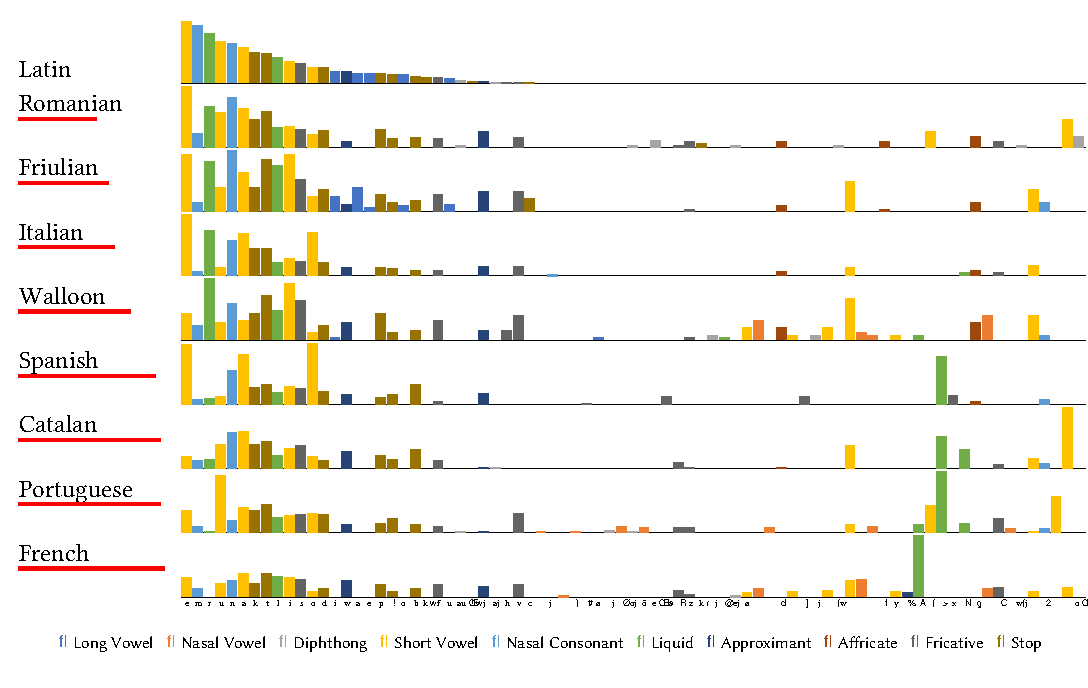
\includegraphics[width=495.9pt]{Figures/SegmentOccuranceRates.pdf}
\caption{Comparison of segmental occurrence rates across languages. Segments are ordered according to their frequency in Latin. For each language, bar heights are normalized to the most frequent segment in that language. Languages are arranged by increasing Euclidean distance from Latin (indicated by the red line). }
\label{SegmentOccuranceRates}
\end{figure*}

The results reported here are derived from a model in which segmental change is represented as a sequence of independent insertion, deletion, and substitution events operating on individual segments. As a consequence, certain types of sound change are not naturally accommodated within this framework. Metathesis, for example---where two segments exchange positions---is not modeled as a single transition. Friulian /tarɔnt/ ultimately derives from Latin /rotundum/ ‘round’, with the initial Latin sequence /rVt/ corresponding to /tVr/ in Friulian. Under TKF91, such a change is represented as two independent substitutions (/r/$\rightarrow$/t/ and /t/$\rightarrow$/r/), rather than as a single reordering event. A second limitation concerns contextual conditioning: transition rates are estimated independently of phonological environment, even though segmental change is often sensitive to adjacent sounds. Finally, the current implementation does not incorporate suprasegmental structure. Features such as stress, which are known to be central to Romance phonological developments, are therefore excluded from the model. 

\subsection{Advantages of the Event-Based Approach}
\label{PaperSections_Advantages}
Despite these limitations, the event-based formulation offers distinct advantages. Since segmental change is modeled explicitly as a stochastic process, it becomes possible to investigate questions that are difficult to address within traditional frameworks. For example, one may ask whether the frequency of a phoneme influences its diachronic stability, how rates of change depend on the size and composition of a phonemic inventory, or to what extent natural classes constrain evolutionary trajectories. Such hypotheses can be evaluated formally through comparisons among models that differ in their parameterization of substitution rates. 

More broadly, embedding sound change within a statistical framework enables both parameter estimation and principled model comparison. Competing hypotheses about linguistic evolution can be formalized as alternative probabilistic models and evaluated using standard inferential criteria. This strategy mirrors the development of molecular evolutionary theory, where increasingly realistic models have been proposed and tested against simpler alternatives. By adopting a similar model-based approach, historical linguistics gains a systematic means of assessing the explanatory adequacy of competing accounts of sound change. 

\section{Conclusion}
\label{PaperSections_Conclusion}
This study provides the first application of the TKF91 model to a linguistic dataset and demonstrates the advantages of modeling language change as a sequence of explicitly defined events. By operating directly on segmental forms rather than abstract cognate relationships, the framework preserves the signal in word forms and permits inference about the dynamics of sound change. The framework can, in principle, be extended to accommodate more complex forms of segmental change, including context-dependent processes. An event-based approach may also improve divergence-time estimation, which depends on quantifying the number of evolutionary events along the branches of a tree. When divergence times are estimated from abstract cognate characters, the nature of these events is often unclear. By contrast, the present model counts explicitly defined operations (segmental substitutions, insertions, and deletions) and thereby provides a more transparent basis for phylogenetic inference. 

The code and data for this study are available on \href{https://github.com/jhuelsenbeck/Linguistomics}{GitHub}. 

\section{Acknowledgements}
\label{PaperSections_Acknowledgements}
We thank Gerton Lunter for guidance on the implementation of the TKF91 model. Earlier versions of this work were presented at the Computational Phylogenetics and Language (Pre)history Workshop in Rethymno, EvoLang 2024, and the UCLA Phonology Seminar. We are grateful to the audiences at these three venues for their valuable feedback, and especially to Chundra Cathcart, Frederik Hartmann, Simon Greenhill, and Gerhard J\"{a}ger for their thoughtful comments. We also thank the three anonymous reviewers for insightful crticism, which substantially improved the paper.


\bibliographystyle{abbrvnat}
\bibliography{main}

\end{document}

